% Options for packages loaded elsewhere
\PassOptionsToPackage{unicode}{hyperref}
\PassOptionsToPackage{hyphens}{url}
%
\documentclass[
]{article}
\usepackage{amsmath,amssymb}
\usepackage{lmodern}
\usepackage{iftex}
\ifPDFTeX
  \usepackage[T1]{fontenc}
  \usepackage[utf8]{inputenc}
  \usepackage{textcomp} % provide euro and other symbols
\else % if luatex or xetex
  \usepackage{unicode-math}
  \defaultfontfeatures{Scale=MatchLowercase}
  \defaultfontfeatures[\rmfamily]{Ligatures=TeX,Scale=1}
\fi
% Use upquote if available, for straight quotes in verbatim environments
\IfFileExists{upquote.sty}{\usepackage{upquote}}{}
\IfFileExists{microtype.sty}{% use microtype if available
  \usepackage[]{microtype}
  \UseMicrotypeSet[protrusion]{basicmath} % disable protrusion for tt fonts
}{}
\makeatletter
\@ifundefined{KOMAClassName}{% if non-KOMA class
  \IfFileExists{parskip.sty}{%
    \usepackage{parskip}
  }{% else
    \setlength{\parindent}{0pt}
    \setlength{\parskip}{6pt plus 2pt minus 1pt}}
}{% if KOMA class
  \KOMAoptions{parskip=half}}
\makeatother
\usepackage{xcolor}
\usepackage[margin=1in]{geometry}
\usepackage{graphicx}
\makeatletter
\def\maxwidth{\ifdim\Gin@nat@width>\linewidth\linewidth\else\Gin@nat@width\fi}
\def\maxheight{\ifdim\Gin@nat@height>\textheight\textheight\else\Gin@nat@height\fi}
\makeatother
% Scale images if necessary, so that they will not overflow the page
% margins by default, and it is still possible to overwrite the defaults
% using explicit options in \includegraphics[width, height, ...]{}
\setkeys{Gin}{width=\maxwidth,height=\maxheight,keepaspectratio}
% Set default figure placement to htbp
\makeatletter
\def\fps@figure{htbp}
\makeatother
\setlength{\emergencystretch}{3em} % prevent overfull lines
\providecommand{\tightlist}{%
  \setlength{\itemsep}{0pt}\setlength{\parskip}{0pt}}
\setcounter{secnumdepth}{-\maxdimen} % remove section numbering
\ifLuaTeX
  \usepackage{selnolig}  % disable illegal ligatures
\fi
\IfFileExists{bookmark.sty}{\usepackage{bookmark}}{\usepackage{hyperref}}
\IfFileExists{xurl.sty}{\usepackage{xurl}}{} % add URL line breaks if available
\urlstyle{same} % disable monospaced font for URLs
\hypersetup{
  pdftitle={Final Project: Predicting Flight Delays using Flight Characteristics and Weather Data},
  pdfauthor={Oliver Ryder-Green},
  hidelinks,
  pdfcreator={LaTeX via pandoc}}

\title{Final Project: Predicting Flight Delays using Flight
Characteristics and Weather Data}
\author{Oliver Ryder-Green}
\date{2022-11-25}

\begin{document}
\maketitle

\clearpage

\section{Introduction}

To paraphrase a well-known idiom, `nothing is certain but death, taxes,
and delayed flights.' Flight delays are an inconvenience that almost all
aviation passengers will experience at some point in their travels. Yet
the burden of flight delays is not the same for all passengers. In
particular, US passengers are not entitled to compensation for
delays\footnote{source:www.transportation.gov}. Yet, between 2013 and
2022, approximately one in every five flights from US airports was
delayed by at least 15 minutes\footnote{source:www.bts.gov}. With more
than 10 million scheduled passenger flights in the US each
year\footnote{source:www.faa.gov}, the cost to passengers of flight
delays is substantial. Indeed, the
\textit{Federal Aviation Administration} estimates that flight delays in
the US from 2016 to 2019 cost US\$62.6billion in total. Short of relying
on airlines to inform them of expected delays (as late as 30 minutes
before scheduled departure), there is little that US passengers can do
to reliably avoid flight delays. Therefore, I apply the classification
methods discussed in class to determine what factors passengers might
consider to avoid flight departure delays. I also consider the extent to
which these factors are able to predict the length of departure delays
that passengers might experience.\\

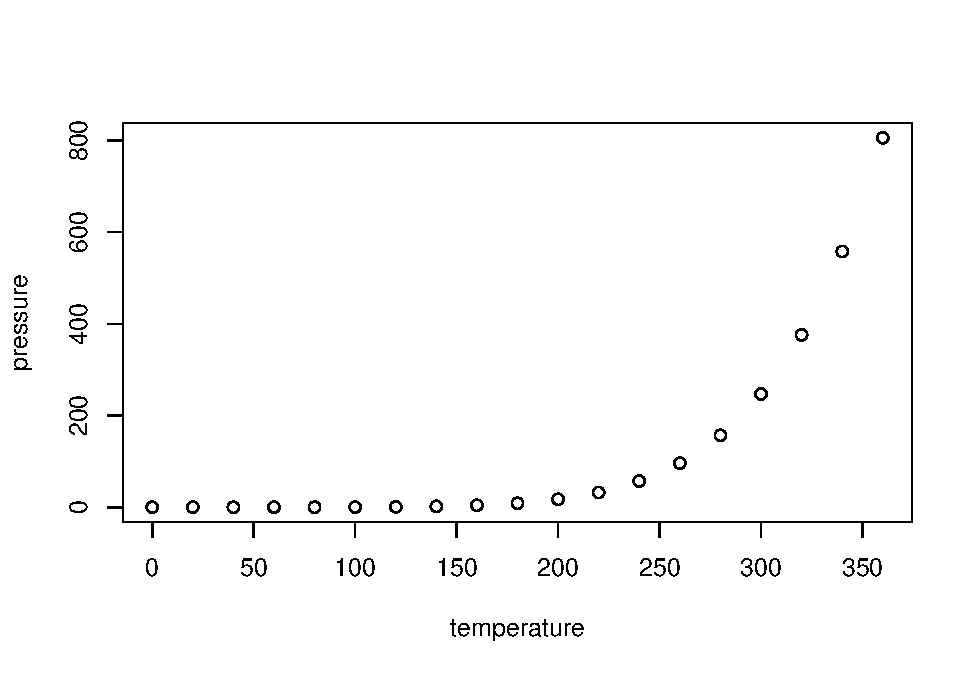
\includegraphics{Visualisation_Analysis_files/figure-latex/pressure-1.pdf}

\end{document}
